\documentclass{article}

\usepackage{booktabs}
\usepackage{microtype}
\usepackage{pgfplots}
\title{Mandatory Assignment 1}
\author{Kris-Mikael Krister (krismikk)\\\texttt{krismikael@protonmail.com}}
\date{\today}

\begin{document}

\maketitle
\section*{Exhaustive Search}

This section describes the results using an exhaustive search implementation for finding the shortest path of a set of cities, also known as the travelling salesman problem. Since an exhaustive search verifies all possible permutations, the algorithm is guaranteed to find the shortest path. See

From the set of the following ten cities, the path found to be shortest is Copenhagen $\rightarrow$ Hamburg $\rightarrow$ Brussels $\rightarrow$ Dublin $\rightarrow$ Barcelona $\rightarrow$ Belgrade $\rightarrow$ Istanbul $\rightarrow$ Bucharest $\rightarrow$ Budapest $\rightarrow$ Berlin. The total distance for the route is 7486.31 km.\\

\noindent The solution was found using 21.25 seconds on a Linux i5-4670 CPU @ 3.40GHz. A single core was used when running the program, so exploiting the multi-core architecture would be a possible improvement to the program.\\

\begin{center}
\begin{tabular}{crr}
\toprule
Number of cities & Permutations & Execution time (seconds) \\
\midrule
$5$ & $120$ & $0.000349998474121$ \\
$6$ & $720$ & $0.00444889068604$ \\
$7$ & $5\,040$ & $0.0201399326324$ \\
$8$ & $40\,320$ & $0.219367980957$ \\
$9$ & $362\,880$ & $1.87963008881$ \\
$10$ & $3\,628\,800$ & $21.25$ \\
$11$ & $39\,916\,800$ & $258$ \\
$12$ & $479\,001\,600$ & $3406.87$ \\
\bottomrule
\end{tabular}
\end{center}

\noindent Difference in execution time corresponds to the number of permutations. The amount of permutations is factorial ($O(n!)$), so based on the results above, the expected running time for all 24 cities would be approximately $3406.87 * 13 * 14 * 15 * 16 * 17 * 18 * 19 * 20 * 21 * 22 * 23 * 24 \approx 4.41 \times 10^{18}$ seconds.

\subsection*{How to run the program}

Execute the \texttt{tsp\_exhaustive.py} file with the amount of cities to check.

\begin{verbatim}
$ python tsp_exhaustive.py 5

Exhastive search using 5 first cities
Found shortest {'distance': 4983.38, 'route': ('Barcelona',
'Belgrade', 'Bucharest', 'Berlin', 'Brussels')} in
time 0.00048303604126
\end{verbatim}

\noindent All modules have one or more unit tests to verify the implementation. To run all tests, use Python's unittest discovery:

\begin{verbatim}
$ python -m unittest discover -p '*_test.py'
\end{verbatim}

\section*{Hill Climber}

This section describes the results using a hill climber implementation to find the shortest path.

\subsection*{Implementation}

Key properties for the implementation are shown below.

\begin{itemize}
    \item A random permutation (route) is chosen as a starting point for the algorithm.
    \item The total route distance for the route is calculated.
    \item The position of two random cities in the route are swapped and the route distance is calculated.
    \item If the new route distance is shorter than the previous one, update the pointer of the best route.
    \item Repeat until the maximum amount of total iterations are reached (set to 5000), or maximum amount of iterations (set to 50) with a change below a threshold (300) is reached.
\end{itemize}

\subsection*{Results}

The algorithm is stochastic and the result can differ between each run. Multiple iterations of the hill climber algorithm must therefore run to be able to compare it to the exhaustive search algorithm. Twenty iterations were used for the comparison.

\begin{center}
\begin{tabular}{lcc}
\toprule
Measurement & Ten cities & All cities \\
\midrule
Best & $7\,486.31$ & $127\,59.8$ \\
Worst & $8\,407.18$ & $15\,209.07$ \\
Mean & $7\,747.34$ & $14\,005.63$ \\
Standard deviation & $346.35$ & $821.67$ \\
\bottomrule
\end{tabular}
\end{center}

The hill climber found the optimal solution for the case of the ten cities (the optimal solution was found with the exhaustive search). The optimal solution for all cities is unknown.

\subsection*{How to run the program}

Execute the \texttt{tsp\_hill\_climber.py} file with the amount of cities to check. Note that Python 3.4 or later is required due to usage of the statistics library for standard deviation.

\begin{verbatim}
$ python tsp_hill_climber.py 24

Hill climber search using first 24 cities. Running in total 20
iterations.
Best   12759.8
Worst  15209.069999999998
Mean   14005.635999999999
stdev  821.6690607307211
\end{verbatim}


\section*{Genetic Algorithm}

This section describes the results using a genetic algorithm for finding the shortest path. This is a permutation problem, so the crossover and mutation operators must be chosen accordingly. The phenotype space is the set of city names. The crossover algorithm used is partial mapped crossover that supports array of city names as input, so the genotype is the same as the phenotype.

\subsection*{Implementation}

The genetic algorithm runs three rounds, with population size set to 50 the first round, 100 for the second and 200 for the third. Number of executions for each round is set to 20 and the best of these exeuctions is used. Each execution has 100 generations.

As with the previous tasks, all individuals in the population are \textit{routes}, e.g. Berlin $\rightarrow$ Barcelona $\rightarrow$ $\ldots$ $\rightarrow$ Belgrade. Each individual has the same number of cities (genes). The general steps for the implementation are shown below.

\begin{enumerate}
    \item An initial population is randomly generated.
    \item The fitness for each individual is calculated. The fitness is based on the total route distance for the individual, compared to the total route distance for the entire population. The shortest route will have the highest fitness.
    \item The number of parents is set to half the population size, and parents are chosen using a stochastic universal sampling (SUS) method to avoid selection bias.
    \item Offspring is created using a partial mapped crossover algorithm. The number of offspring is set to double the amount of the population.
    \item The mutation strategy is \textit{swap two genes} up to two times per child. The initial mutation strategy was swap up to one time with probability $50\%$, but had to be adjusted as the population in that case in almost all cases converged towards having the same fitness. Mutation probablity $60\%$ plus a second round of swap with probability $40\%$ elliminated this symptom in all cases I tested.
    \item A $\mu,\lambda$ selection is used to form the next generation. All parents are discarded, and the fittest half of the $2 \times \lambda$ offspring are selected for the next generation.
\end{enumerate}

\subsection*{Results}

The results shows the best run of the 20 executions for each of the three population sizes.

\subsubsection*{Population size 50}

\begin{center}
\begin{tabular}{lcc}
\toprule
Measurement & Ten cities & All cities \\
\midrule
Best & $7\,486.31$ km & $12\,976.68$ km \\
Worst & $7\,503.10$ & $17\,288.78$ \\
Mean & $7\,488.82$ & $14\,086.72$ \\
Standard deviation & $6.15$ & $990.21$ \\
Execution time & $3.64$ s & $7.99$ s \\
\bottomrule
\end{tabular}
\end{center}

\subsubsection*{Population size 100}

\begin{center}
\begin{tabular}{lcc}
\toprule
Measurement & Ten cities & All cities \\
\midrule
Best & $7\,486.31$ km & $12\,287.07$ km \\
Worst & $7\,503.10$ & $15\,964.22$ \\
Mean & $7\,487.99$ & $13\,794.15$ \\
Standard deviation & $5.17$ & $1\,032.31$ \\
Execution time & $7.44$ s & $16.18$ s \\
\bottomrule
\end{tabular}
\end{center}

\subsubsection*{Population size 200}

\begin{center}
\begin{tabular}{lcc}
\toprule
Measurement & Ten cities & All cities \\
\midrule
Best & $7\,486.31$ km & $12\,771.46$ km \\
Worst & $7\,486.31$ & $14\,567.73$ \\
Mean & $7\,486.31$ & $13\,581.41$ \\
Standard deviation & $\approx 0$ & $396.53$ \\
Execution time & $15.33$ s & $33.12$ s \\
\bottomrule
\end{tabular}
\end{center}

% arstr.replace(/\s+/g, ' ').trim().split(' ').map((elem, index) => `(${index},${elem})`).join('')

Noter noe om at alle 10-city med pop 100+ fant den riktige verdien

Avg over tre populasjoner med best i hver generasjon (10 byer):

\subsubsection*{Average values}

The following graph shows the best value in average for each generation when calculating shortest route for 10 cities.

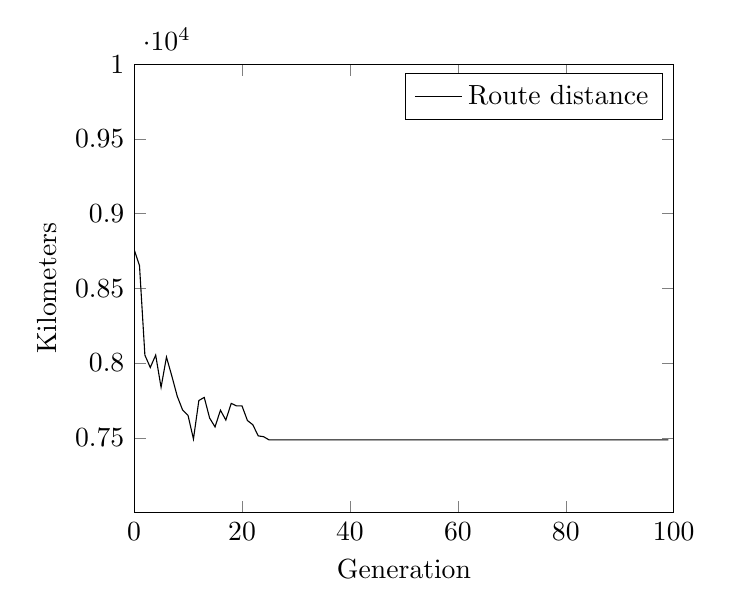
\begin{tikzpicture}
\begin{axis}[
    xlabel={Generation},
    ylabel={Kilometers},
    xmin=0, xmax=100,
    ymin=7000, ymax=10000,
    xtick={0,20,40,60,80,100},
    ytick={7500,8000,8500,9000,9500,10000}
]
\addplot[
]
coordinates {
    (0,8761.17333333)(1,8653.04666667)(2,8053.13333333)(3,7970.54333333)(4,8053.19666667)(5,7837.73333333)(6,8040.15)(7,7912.34333333)(8,7777.68666667)(9,7685.17666667)(10,7649.14333333)(11,7491.90666667)(12,7749.42666667)(13,7770.31333333)(14,7631.87333333)(15,7572.80666667)(16,7684.61)(17,7618.90333333)(18,7730.25333333)(19,7713.13666667)(20,7713.13666667)(21,7615.7)(22,7587.34)(23,7512.85666667)(24,7507.26)(25,7486.31)(26,7486.31)(27,7486.31)(28,7486.31)(29,7486.31)(30,7486.31)(31,7486.31)(32,7486.31)(33,7486.31)(34,7486.31)(35,7486.31)(36,7486.31)(37,7486.31)(38,7486.31)(39,7486.31)(40,7486.31)(41,7486.31)(42,7486.31)(43,7486.31)(44,7486.31)(45,7486.31)(46,7486.31)(47,7486.31)(48,7486.31)(49,7486.31)(50,7486.31)(51,7486.31)(52,7486.31)(53,7486.31)(54,7486.31)(55,7486.31)(56,7486.31)(57,7486.31)(58,7486.31)(59,7486.31)(60,7486.31)(61,7486.31)(62,7486.31)(63,7486.31)(64,7486.31)(65,7486.31)(66,7486.31)(67,7486.31)(68,7486.31)(69,7486.31)(70,7486.31)(71,7486.31)(72,7486.31)(73,7486.31)(74,7486.31)(75,7486.31)(76,7486.31)(77,7486.31)(78,7486.31)(79,7486.31)(80,7486.31)(81,7486.31)(82,7486.31)(83,7486.31)(84,7486.31)(85,7486.31)(86,7486.31)(87,7486.31)(88,7486.31)(89,7486.31)(90,7486.31)(91,7486.31)(92,7486.31)(93,7486.31)(94,7486.31)(95,7486.31)(96,7486.31)(97,7486.31)(98,7486.31)(99,7486.31)
};
\legend{Route distance}
\end{axis}
\end{tikzpicture}


The following graph shows the best value in average for each generation when calculating shortest route for 24 cities.

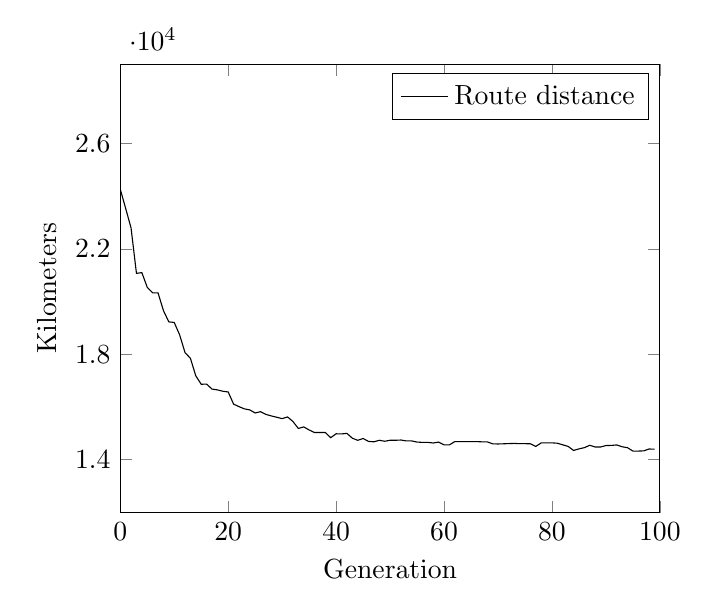
\begin{tikzpicture}
\begin{axis}[
    xlabel={Generation},
    ylabel={Kilometers},
    xmin=0, xmax=100,
    ymin=12000, ymax=29000,
    xtick={0,20,40,60,80,100},
    ytick={14000,18000,22000,26000}
]
\addplot[
]
coordinates {
    (0,24262.53666667)(1,23532.69666667)(2,22792.76)(3,21068.52666667)(4,21097.56)(5,20541.21666667)(6,20329.74666667)(7,20329.74666667)(8,19657.55666667)(9,19228.71333333)(10,19207.2)(11,18739.79333333)(12,18064.93)(13,17847.37333333)(14,17180.91666667)(15,16864.02)(16,16869.42333333)(17,16680.98)(18,16650.8)(19,16598.36333333)(20,16572.02333333)(21,16111.1)(22,16015.06)(23,15930.62666667)(24,15890.63)(25,15774.97666667)(26,15823.85666667)(27,15720.61)(28,15661.66)(29,15612.65666667)(30,15560.02)(31,15624.99333333)(32,15450.73)(33,15187.18333333)(34,15245.30666667)(35,15130.53666667)(36,15033.34666667)(37,15033.34666667)(38,15033.34666667)(39,14837.58333333)(40,14985.53666667)(41,14979.47)(42,15002.23666667)(43,14818.79666667)(44,14737.81333333)(45,14807.00666667)(46,14696.78)(47,14681.09666667)(48,14739.08)(49,14701.81666667)(50,14739.08)(51,14739.08)(52,14749.15)(53,14715.01)(54,14715.01)(55,14671.05333333)(56,14659.17)(57,14659.17)(58,14635.78666667)(59,14671.05333333)(60,14565.74333333)(61,14565.74333333)(62,14690.33333333)(63,14690.33333333)(64,14690.33333333)(65,14690.33333333)(66,14690.33333333)(67,14680.16666667)(68,14680.16666667)(69,14605.61666667)(70,14598.81)(71,14605.61666667)(72,14614.16)(73,14620.15333333)(74,14611.04)(75,14611.04)(76,14605.61666667)(77,14505.73)(78,14638.82666667)(79,14638.82666667)(80,14642.46)(81,14626.95666667)(82,14566.81666667)(83,14507.73333333)(84,14353.58333333)(85,14412.59)(86,14459.44666667)(87,14549.70666667)(88,14484.55333333)(89,14484.55333333)(90,14539.06)(91,14544.45333333)(92,14562.16666667)(93,14493.5)(94,14457.81)(95,14329.78666667)(96,14329.78666667)(97,14337.27)(98,14408.49)(99,14401.00666667)
};
\legend{Route distance}
\end{axis}
\end{tikzpicture}


Alle tre verdier (24 byer)

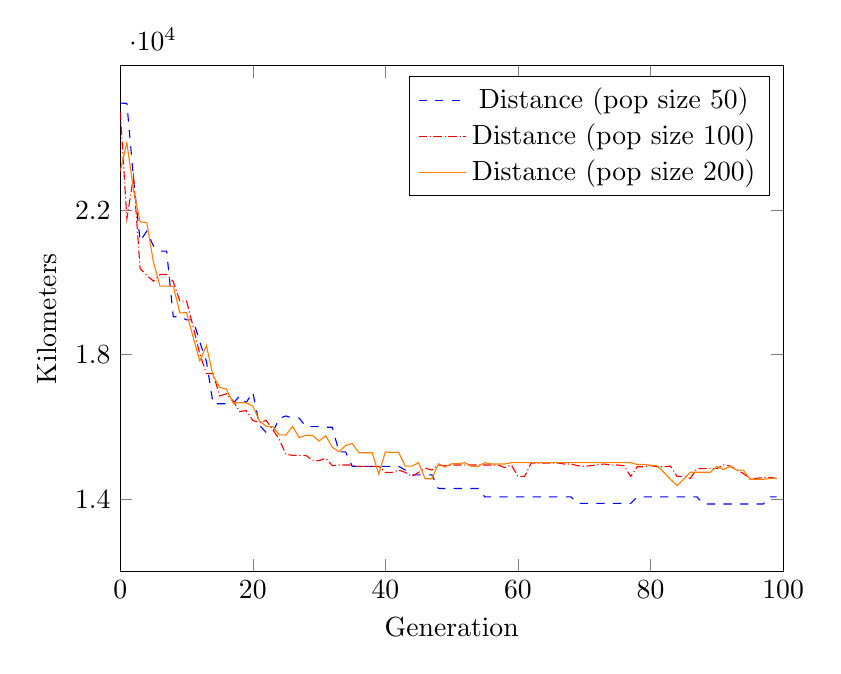
\begin{tikzpicture}
\begin{axis}[
    xlabel={Generation},
    ylabel={Kilometers},
    xmin=0, xmax=100,
    ymin=12000, ymax=26000,
    xtick={0,20,40,60,80,100},
    width=10cm, height=8cm,
    ytick={14000,18000,22000}
]
\addplot[
color=blue,
dashed
]
coordinates {
    (0,24969.59)(1,24962.659999999996)(2,22875.34)(3,21144.85)(4,21423.31000000001)(5,21014.899999999998)(6,20867.690000000002)(7,20867.690000000002)(8,19051.100000000006)(9,19051.100000000006)(10,18965.770000000004)(11,18965.770000000004)(12,18348.340000000004)(13,17816.880000000005)(14,16642.350000000002)(15,16642.350000000002)(16,16642.350000000002)(17,16642.350000000002)(18,16857.290000000005)(19,16674.450000000004)(20,16962.280000000002)(21,16047.140000000003)(22,15848.730000000003)(23,15848.730000000003)(24,16243.280000000002)(25,16303.74)(26,16243.280000000002)(27,16243.280000000002)(28,16006.380000000001)(29,16006.380000000001)(30,16006.380000000001)(31,15990.270000000002)(32,15990.270000000002)(33,15306.86)(34,15306.86)(35,14907.51)(36,14907.51)(37,14907.51)(38,14907.51)(39,14907.51)(40,14907.51)(41,14907.51)(42,14907.51)(43,14805.380000000003)(44,14672.86)(45,14672.86)(46,14672.86)(47,14672.86)(48,14294.740000000002)(49,14294.740000000002)(50,14294.740000000002)(51,14294.740000000002)(52,14294.740000000002)(53,14294.740000000002)(54,14294.740000000002)(55,14060.45)(56,14060.45)(57,14060.45)(58,14060.45)(59,14060.45)(60,14060.45)(61,14060.45)(62,14060.45)(63,14060.45)(64,14060.45)(65,14060.45)(66,14060.45)(67,14060.45)(68,14060.45)(69,13880.41)(70,13880.41)(71,13880.41)(72,13880.41)(73,13880.41)(74,13880.41)(75,13880.41)(76,13880.41)(77,13880.41)(78,14060.45)(79,14060.45)(80,14060.45)(81,14060.45)(82,14060.45)(83,14060.45)(84,14060.45)(85,14060.45)(86,14060.45)(87,14060.45)(88,13864.989999999998)(89,13864.989999999998)(90,13864.989999999998)(91,13864.989999999998)(92,13864.989999999998)(93,13864.989999999998)(94,13864.989999999998)(95,13864.989999999998)(96,13864.989999999998)(97,13864.989999999998)(98,14060.45)(99,14060.45)
};
\addlegendentry{Distance (pop size 50)}
\addplot[
color=red,
densely dashdotted
]
coordinates {
    (0,24735.03)(1,21768.109999999993)(2,22937.209999999995)(3,20380.390000000003)(4,20207.89)(5,20035.300000000003)(6,20220.4)(7,20220.4)(8,20020.420000000002)(9,19477.94)(10,19490.33)(11,18772.030000000002)(12,18018.14)(13,17474.98)(14,17474.98)(15,16857.879999999997)(16,16917.519999999997)(17,16730.91)(18,16425.64)(19,16450.960000000003)(20,16181.06)(21,16113.929999999998)(22,16181.06)(23,15927.759999999998)(24,15650.050000000001)(25,15242.63)(26,15212.9)(27,15212.9)(28,15212.9)(29,15065.89)(30,15065.89)(31,15133.050000000001)(32,14925.16)(33,14943.72)(34,14943.72)(35,14943.72)(36,14907.029999999999)(37,14907.029999999999)(38,14907.029999999999)(39,14907.029999999999)(40,14739.169999999998)(41,14739.169999999998)(42,14807.470000000001)(43,14739.169999999998)(44,14628.74)(45,14739.169999999998)(46,14854.52)(47,14807.470000000001)(48,14943.72)(49,14922.58)(50,14943.72)(51,14943.72)(52,14943.72)(53,14943.72)(54,14943.72)(55,14943.72)(56,14943.72)(57,14943.72)(58,14873.570000000002)(59,14943.72)(60,14627.790000000003)(61,14627.790000000003)(62,15001.56)(63,15001.56)(64,15001.56)(65,15001.56)(66,15001.56)(67,14971.060000000001)(68,14971.060000000001)(69,14927.45)(70,14907.029999999999)(71,14927.45)(72,14953.079999999998)(73,14971.060000000001)(74,14943.72)(75,14943.72)(76,14927.45)(77,14627.790000000003)(78,14896.950000000003)(79,14896.950000000003)(80,14927.45)(81,14896.950000000003)(82,14896.950000000003)(83,14913.220000000001)(84,14627.790000000003)(85,14627.790000000003)(86,14574.84)(87,14845.62)(88,14845.62)(89,14845.62)(90,14845.62)(91,14948.61)(92,14916.240000000002)(93,14813.95)(94,14706.880000000001)(95,14574.84)(96,14574.84)(97,14597.290000000005)(98,14597.290000000005)(99,14574.84)
};
\addlegendentry{Distance (pop size 100)}
\addplot[
color=orange,
]
coordinates {
    (0,23082.989999999998)(1,23867.320000000003)(2,22565.729999999996)(3,21680.340000000004)(4,21661.48)(5,20573.450000000004)(6,19901.15)(7,19901.15)(8,19901.15)(9,19157.099999999995)(10,19165.499999999996)(11,18481.58)(12,17828.31)(13,18250.260000000002)(14,17425.420000000002)(15,17091.83)(16,17048.4)(17,16669.68)(18,16669.47)(19,16669.68)(20,16572.73)(21,16172.230000000001)(22,16015.39)(23,16015.39)(24,15778.560000000001)(25,15778.560000000001)(26,16015.39)(27,15705.650000000001)(28,15765.7)(29,15765.7)(30,15607.789999999999)(31,15751.66)(32,15436.76)(33,15310.97)(34,15485.34)(35,15540.380000000001)(36,15285.5)(37,15285.5)(38,15285.5)(39,14698.21)(40,15309.93)(41,15291.73)(42,15291.73)(43,14911.84)(44,14911.84)(45,15008.989999999998)(46,14562.959999999997)(47,14562.959999999997)(48,14978.779999999999)(49,14888.130000000001)(50,14978.779999999999)(51,14978.779999999999)(52,15008.989999999998)(53,14906.57)(54,14906.57)(55,15008.989999999998)(56,14973.34)(57,14973.34)(58,14973.34)(59,15008.989999999998)(60,15008.989999999998)(61,15008.989999999998)(62,15008.989999999998)(63,15008.989999999998)(64,15008.989999999998)(65,15008.989999999998)(66,15008.989999999998)(67,15008.989999999998)(68,15008.989999999998)(69,15008.989999999998)(70,15008.989999999998)(71,15008.989999999998)(72,15008.989999999998)(73,15008.989999999998)(74,15008.989999999998)(75,15008.989999999998)(76,15008.989999999998)(77,15008.989999999998)(78,14959.079999999998)(79,14959.079999999998)(80,14939.48)(81,14923.470000000001)(82,14743.05)(83,14549.529999999999)(84,14372.509999999998)(85,14549.529999999999)(86,14743.05)(87,14743.05)(88,14743.05)(89,14743.05)(90,14906.57)(91,14819.760000000002)(92,14905.27)(93,14801.560000000001)(94,14801.560000000001)(95,14549.529999999999)(96,14549.529999999999)(97,14549.529999999999)(98,14567.73)(99,14567.73)
};
\addlegendentry{Distance (pop size 200)}
\end{axis}
\end{tikzpicture}

\subsubsection*{Number of generations}

Skriv noe om at det konvergerte mot en løsning og at antall generasjoner ikke trengte å være så høy.

\end{document}
